\chapter{Testing Results}
\label{chapter:results}

%%%%%%%%%%%%%%%%%%%%%%%%% timing %%%%%
\section{Timing}

\begin{table}[h]
	\caption{The table shows the time in seconds to compute the different distances. Take note, that all metrics except the geodesic distance need to have the Laplacian eigenfunctions computed.}
	\begin{tabular}{c*{6}{|r}|}
		$|Vertices|$ &\begin{tabular}{@{}c@{}}Laplacian\\eigenfunctions\\/-values\end{tabular} & diffusion & \begin{tabular}{@{}c@{}}commute\\time\end{tabular}&
		biharmonic & \begin{tabular}{@{}c@{}}geodesic\\exact\end{tabular} & \begin{tabular}{@{}c@{}}geodesic\\Dijkstra\end{tabular}\\
		\hline
		1k  & 2.98   & 0.033 & 0.016 & 0.017 & 0.057  & 0.006 \\
		5k  & 12.46  & 0.122 & 0.064 & 0.070 & 0.481  & 0.014 \\
		10k & 30.35  & 0.283 & 0.157 & 0.169 & 1.449  & 0.036 \\
		20k & 65.08  & 0.487 & 0.268 & 0.288 & 3.632  & 0.063 \\
		50k & 206.58 & 1.193 & 0.655 & 0.705 & 12.123 & 0.149 \\
	\end{tabular}
	\label{tab:timing}
\end{table}

The average computation times to compute the distance from one point to all other points are condensed into table~\ref{tab:timing}.
We can see, that the computation of the Laplacian eigenfunctions and eigenvalues takes the most time.
But after obtaining them, the computation time of the diffusion, the commute-time and the biharmonic distance are really short.
Since they all have the same basic structure, the small differences in speed are results of the different factors:
While the factor $\frac{1}{\lambda_i}$ of the commute-time distance is the fastest to compute, the additional square of the eigenvalue for the biharmonic distance makes it slightly slower.
The fact that the factor of the diffusion distance consists of an exponentiation and a product makes it the slowest one of those three.

One important thing to note here is that even though the computation of the Laplacian eigenfunctions and eigenvalues takes quite a bit of time, the result can be saved and reused every time the distance has to be computed.
So if we were to compute the distance between all points of the mesh (even with respecting the symmetry of the metric and therefore half the computations), the computation of the Laplacian based metrics is already faster then the exact geodesic distance on the mesh with 5000 vertices by an approximate factor of 4.

Even though the implementation of the geodesic is highly optimised, the exact geodesic distance is definitely the slowest metric to compute.
Here the propagation of the windows over all edges of the mesh comes into play.
In the paper \cite{surazhsky2005fast} it is stated, that the windows per edge increase exponentially and, since each new vertex is connected to the rest of the mesh by at least one edge, this means that the computation time has to increase at least at the same speed.
If you approximate the geodesic distance by the Dijkstra algorithm, the computation gets faster than every other metric but its quality decreases significantly.

\section{Sensitivity to noise, tessellation and deformation}

\subsection{Isolines}
\paragraph{The geodesic distance}
\begin{figure}[h]
	\centering
	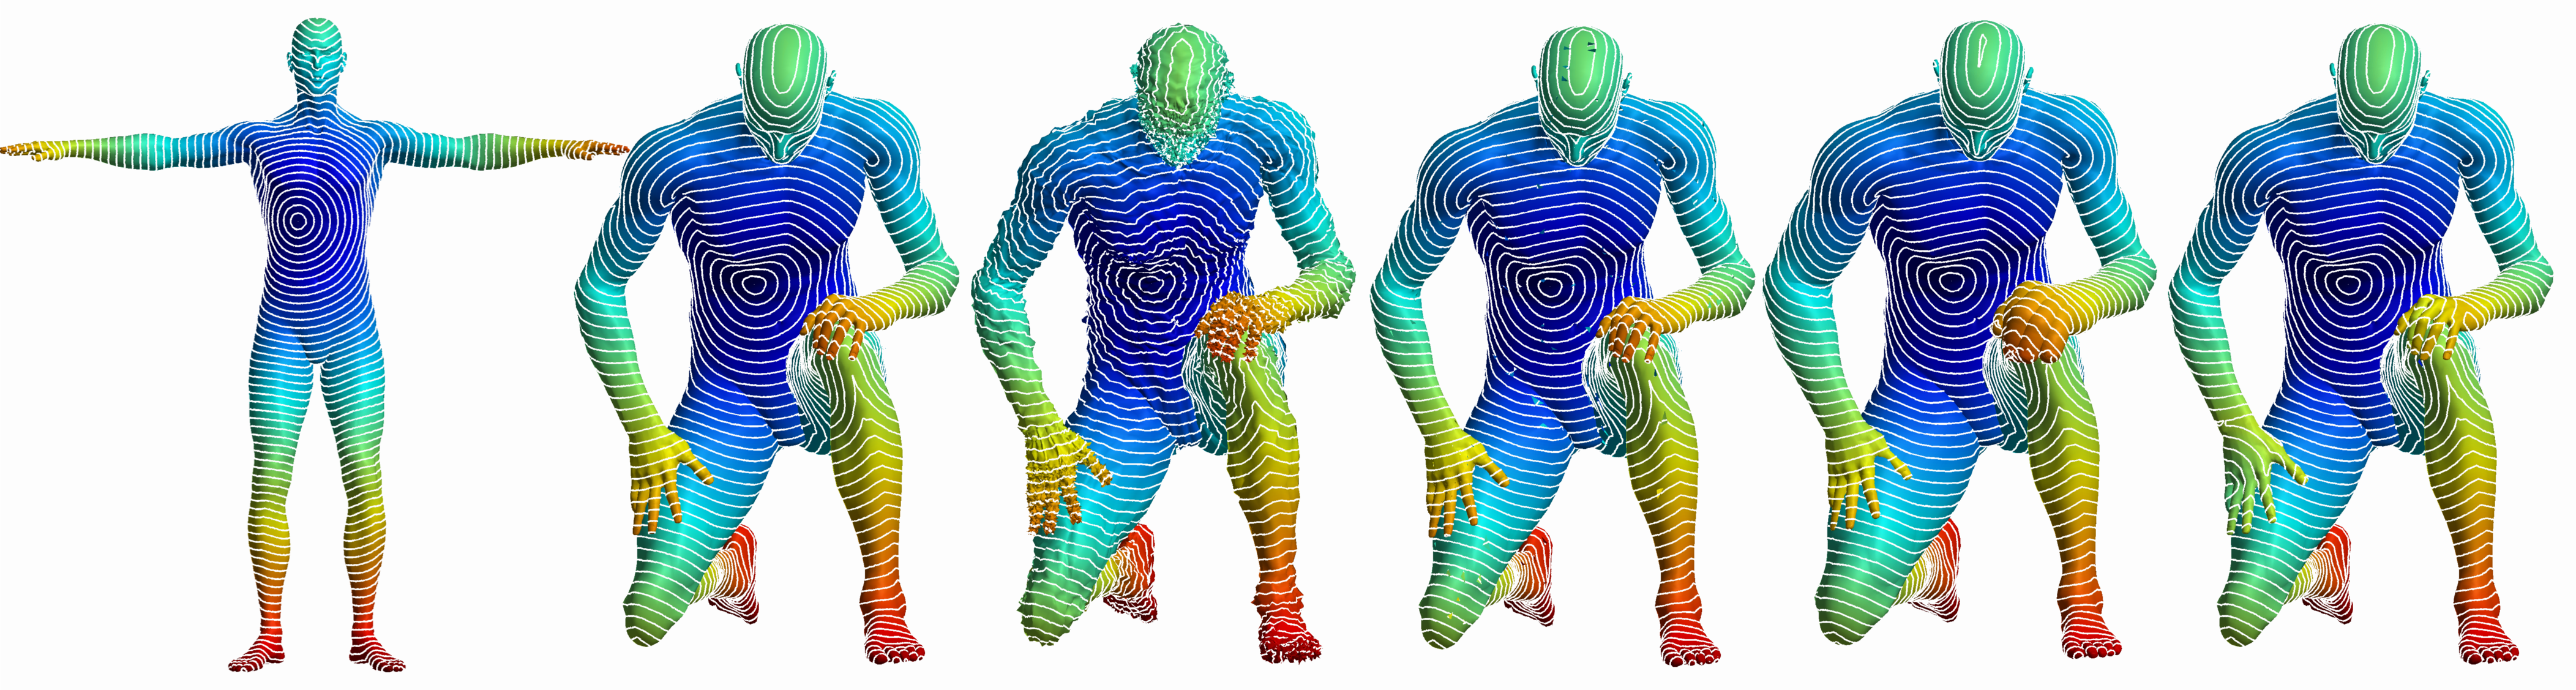
\includegraphics[width = \textwidth]{../results/geodesic_isolines}
	\caption{Comparison of the geodesic distance under different deformations of the mesh; from left to right: the null shape, isometry, noise, microholes, local scaling and topology changes.}
	\label{fig:geo_isolines}
\end{figure}
something else for each one.

\paragraph{The diffusion distance}
\begin{figure}[h]
	\centering
	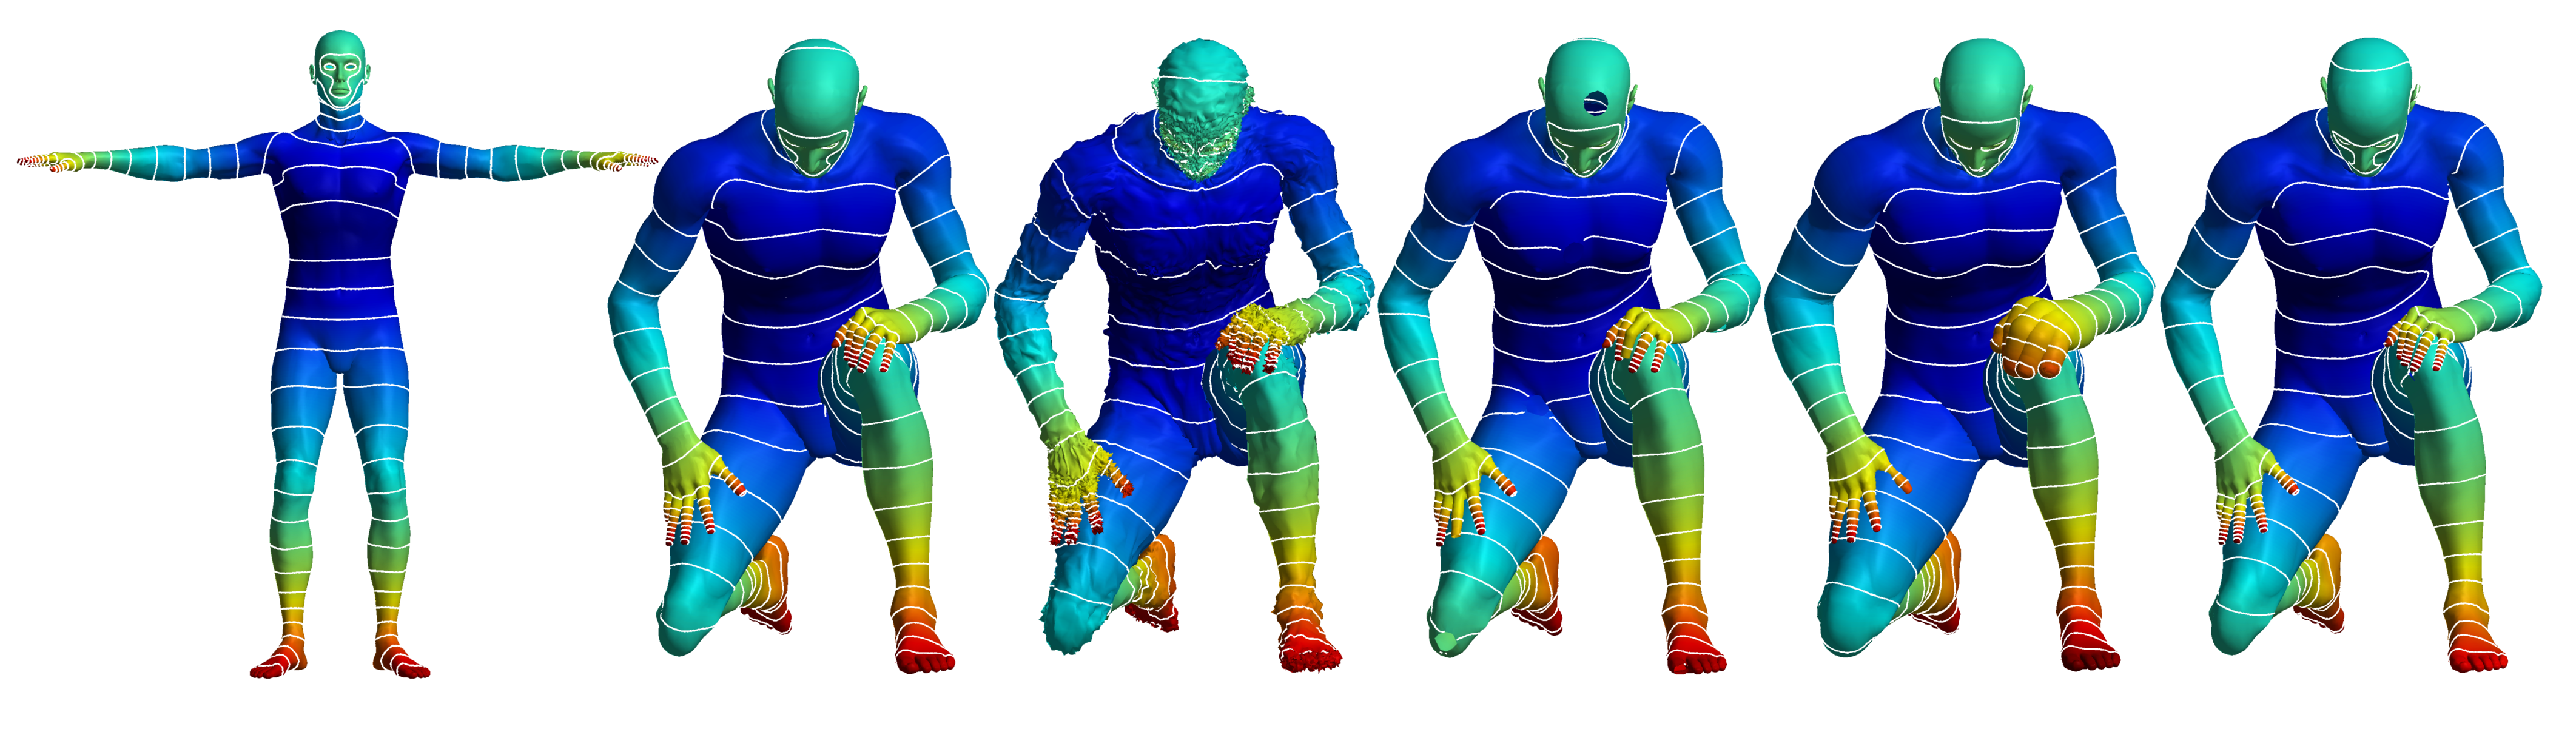
\includegraphics[width = \textwidth]{../results/diffusion_small_isolines}
	\caption{Comparison of the diffusion distance with $t = 0.1$ under different deformations of the mesh; from left to right: the null shape, isometry, noise, holes, local scaling and topology changes.}
	\label{fig:diffusion_s_isolines}
\end{figure}
something for the smaller distances

\begin{figure}[h]
	\centering
	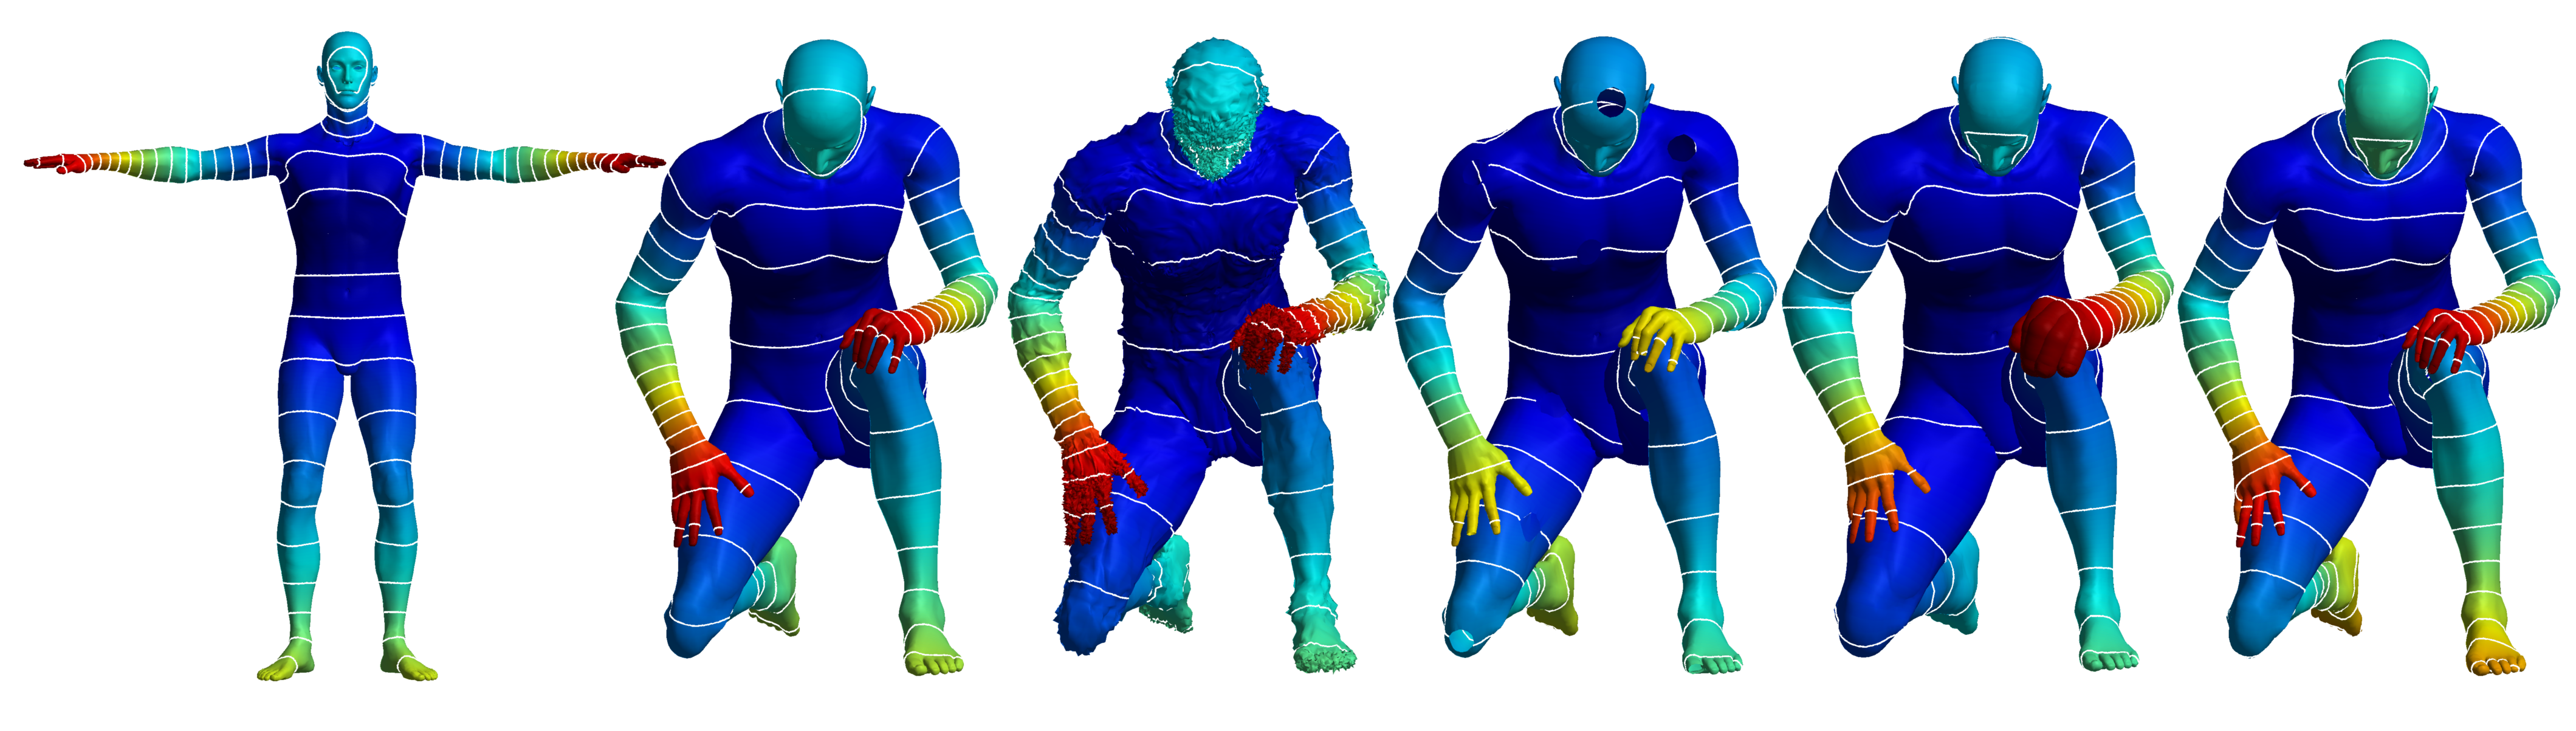
\includegraphics[width = \textwidth]{../results/diffusion_big_isolines}
	\caption{Comparison of the diffusion distance with $t = 1$ under different deformations of the mesh; from left to right: the null shape, isometry, noise, holes, local scaling and topology changes.}
	\label{fig:diffusion_b_isolines}
\end{figure}
something for the bigger distance

\paragraph{The commute-time distance}
\begin{figure}[h]
	\centering
	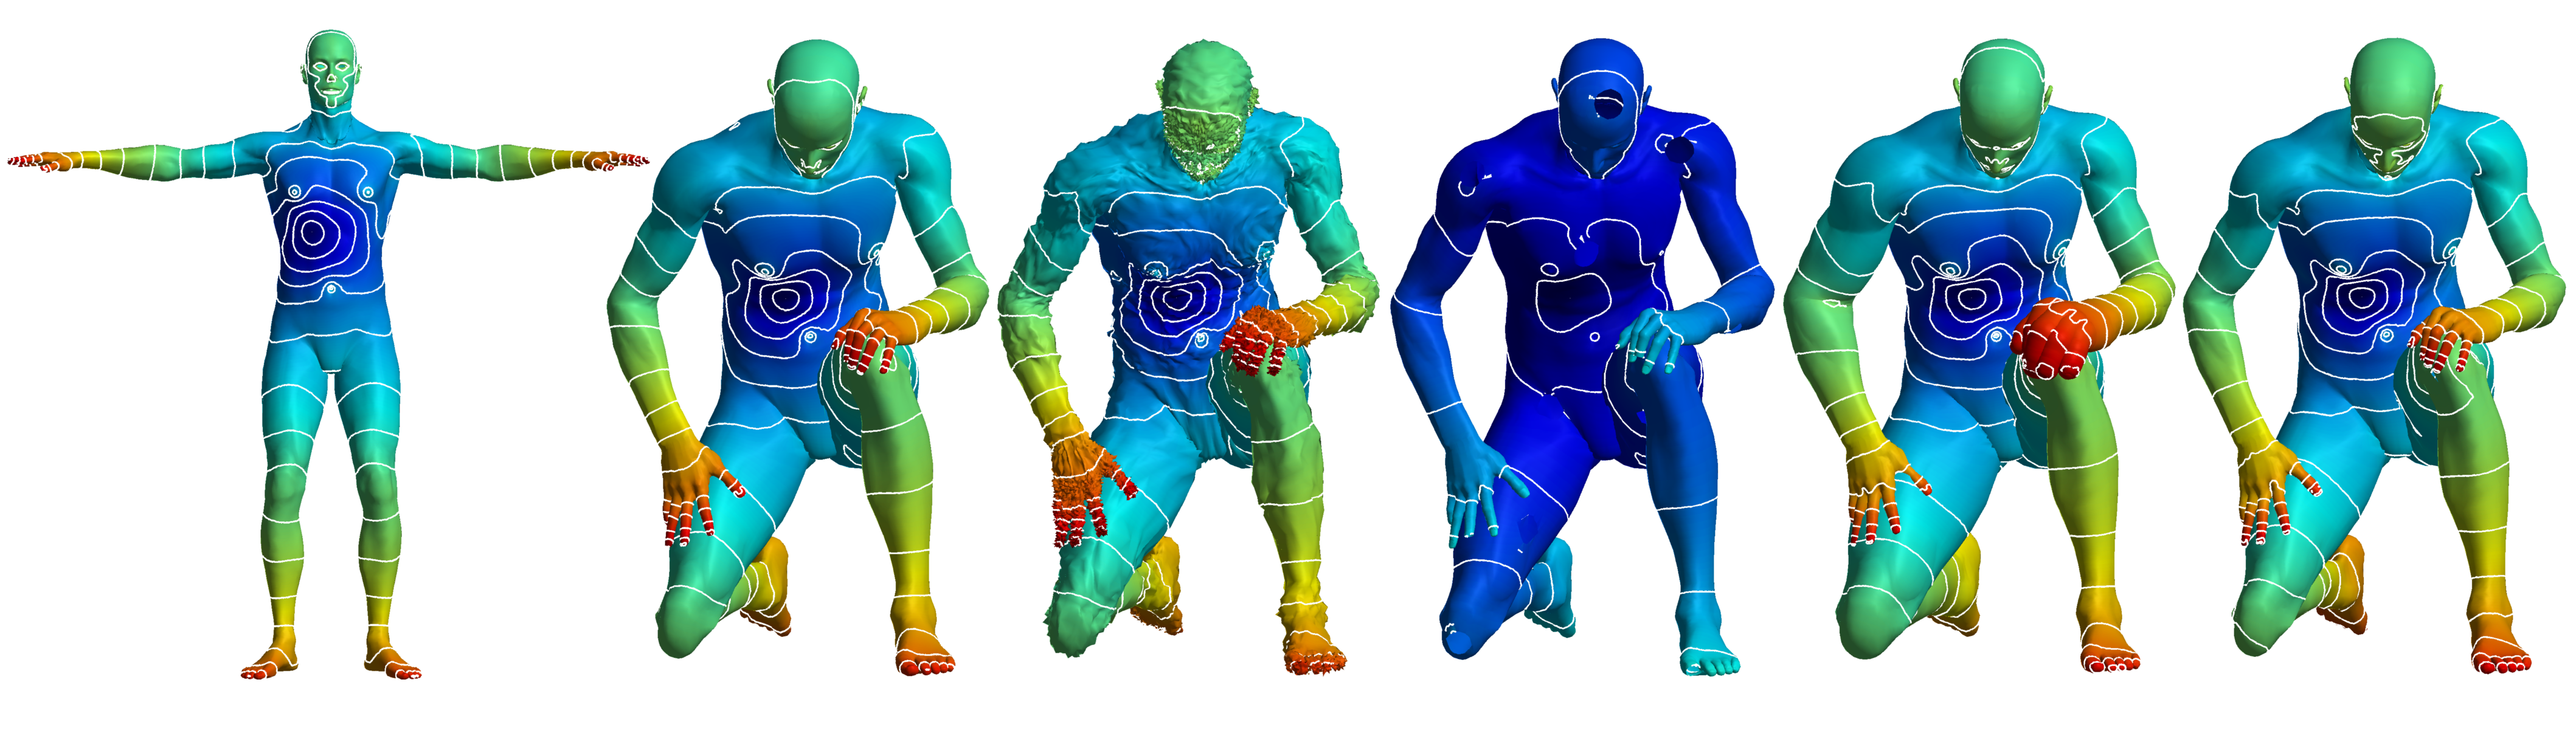
\includegraphics[width = \textwidth]{../results/commute_time_isolines}
	\caption{Comparison of the commute-time distance under different deformations of the mesh; from left to right: the null shape, isometry, noise, holes, local scaling and topology changes.}
	\label{fig:commute_time_isolines}
\end{figure}
something else for each one.

\paragraph{The biharmonic distance}
\begin{figure}[h]
	\centering
	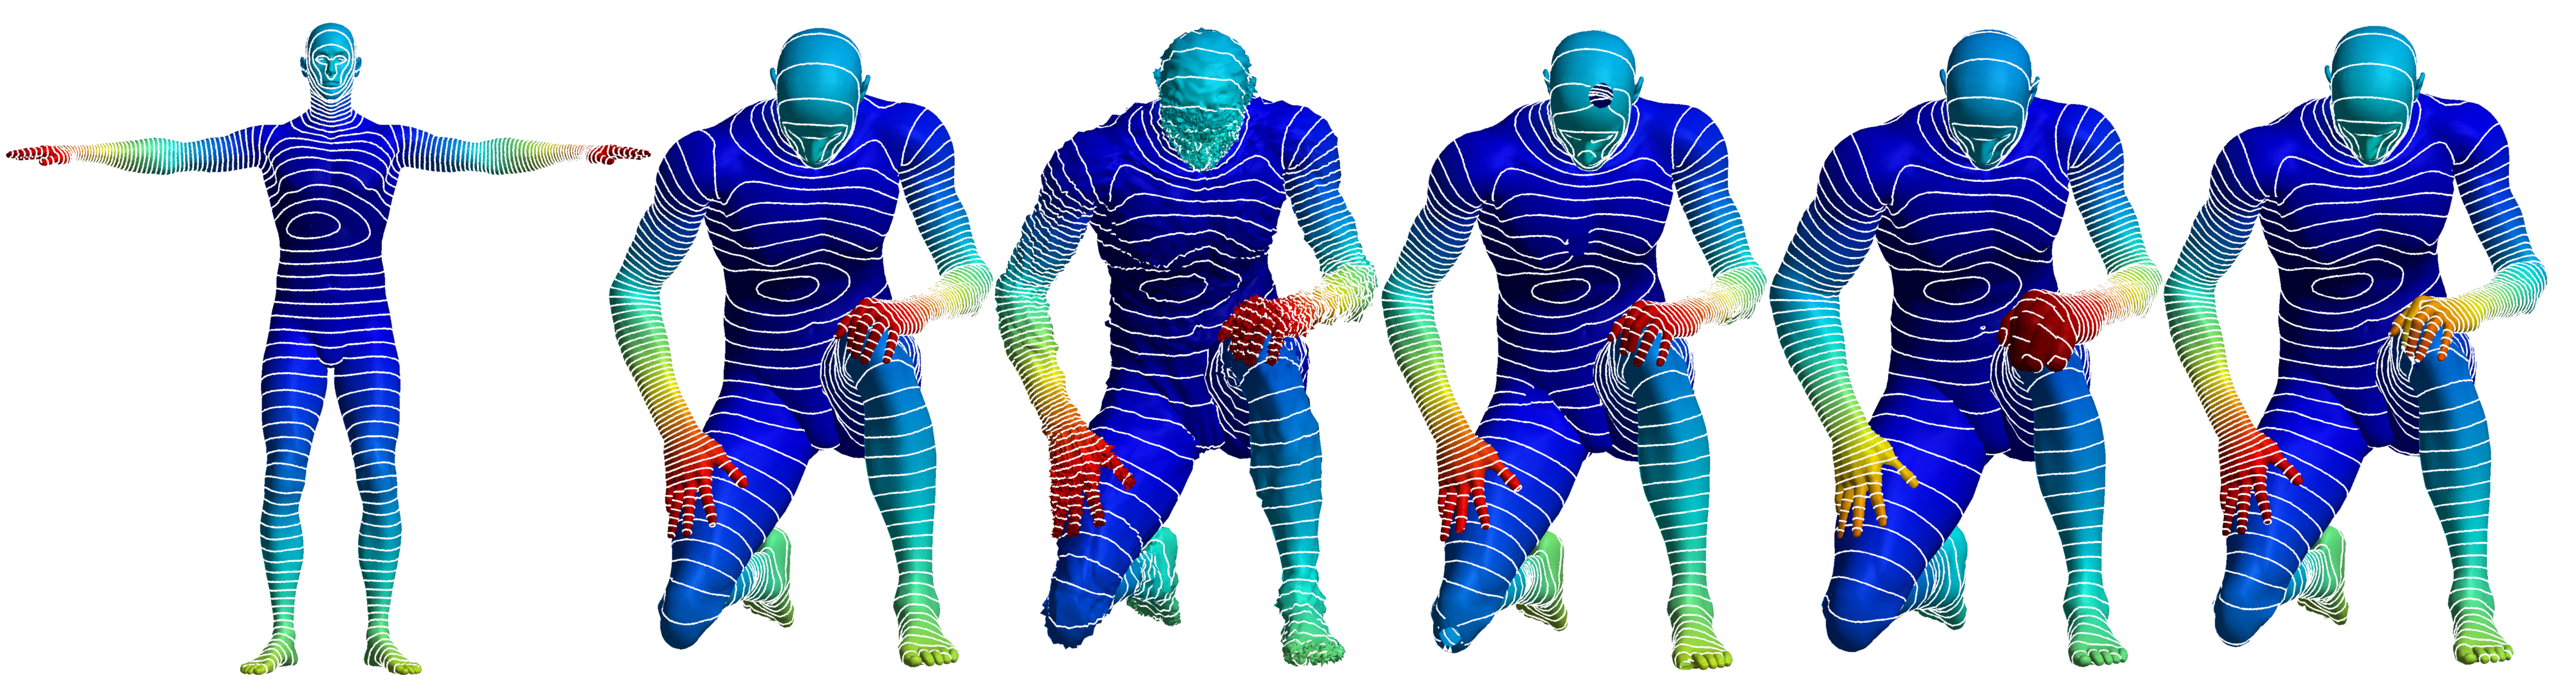
\includegraphics[width = \textwidth]{../results/biharmonic_isolines}
	\caption{Comparison of the biharmonic distance under different deformations of the mesh; from left to right: the null shape, isometry, noise, holes, local scaling and topology changes.}
	\label{fig:biharmonic_isolines}
\end{figure}
something else for each one.

\subsection{FPS}
something

\subsection{Metric distortion}
\begin{table}[h]
	\caption{The mean of the distances, grouped by the type of deformation}
	\begin{tabular}{c*{8}{|r}|}
		metric & isometry & microholes & localscale & noise & scale & topology & shotnoise & holes \\
		\hline
		geodesic & .0232 & .0417 & .0407 & .0218 & .1580 & .0508 & .0419 & - \\
		diffusion t=0.1 & .0043 & .0059 & .0310 & .0241 & .0058 & .0408 & .0044 & .0434 \\
		diffusion t=1 & .0022 & .0031 & .0320 & .0180 & .0029 & .0223 & .0018 & .0528 \\
		commute-time & .0034 & .0035 & .0092 & .0309 & .0037 & .0138 & .0031 & .0331 \\
		biharmonic & .0049 & .0017 & .0220 & .0625 & .0016 & .0420 & .0024 & .0388 \\
	\end{tabular}
	\label{tab:mean}
\end{table}
\begin{table}[h]
	\caption{The max error of the distances, grouped by the type of deformation}
	\begin{tabular}{c*{8}{|r}|}
		metric & isometry & microholes & localscale & noise & scale & topology & shotnoise & holes \\
		\hline
		geodesic & .0984 & .1566 & .1554 & .1311 & .4064 & .2227 & .1567 & - \\
		diffusion t=0.1 & .0258 & .0346 & .2745 & .0728 & .0347 & .0774 & .0365 & .2209 \\
		diffusion t=1 & .0217 & .0302 & .1473 & .0685 & .0301 & .2042 & .0330 & .4938 \\
		commute-time & .0288 & .0469 & .0899 & .1381 & .0493 & .1598 & .0487 & .6374 \\
		biharmonic & .0188 & .0276 & .0648 & .1113 & .0285 & .3226 & .0275 & .5229 \\
	\end{tabular}
	\label{tab:maxerror}
\end{table}

long thing with two tables
